\documentclass{article}

\usepackage{graphicx}
\begin{document}

\title{Presentación del primer proyecto de programación}
\author{Michell Viu Ramirez}
\date{Julio, 2023}
\maketitle

\begin{figure}[h]
    \centering
    
\includegraphics[width=3cm]{matcom.jpg}
\end{figure}

\newpage
\tableofcontents

\newpage
\section{Introducción}
\textbf{¿} Qué es \textit{Moogle!} \textbf{?}\\
Moogle! es una aplicación totalmente original cuyo propósito es buscar 
inteligentemente un texto en un conjunto de documentos.
Es una aplicación web, desarrollada con tecnología .NET Core 6.0, específicamente 
usando Blazor como framework web para la interfaz gráfica, y en el lenguaje C\#.
La idea original del proyecto es buscar en un conjunto de archivos de texto (con extensión `.txt`)

\begin{figure}[h]
    \centering
    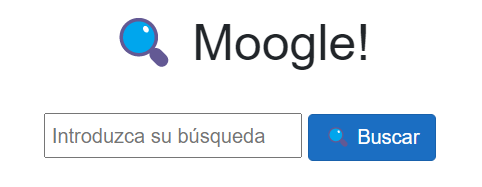
\includegraphics[width=6cm]{Moogle.png}
\end{figure}

\section{Arquitectura del proyecto}
El nuevo proyecto cuenta con cuatro clases nuevas
\begin{itemize}
    \item Clase \textit{Documentos}: Esta clase consta de cinco propiedades y de diez métodos, la propiedad `nombreDocumento` de tipo string que represeta el nombre del "Documento",
    la propiedad `score` de tipo double que representa la relevancia de ese "Documento" para una búsqueda dada, la propiedad `contenido` de tipo string[ ] que representa cada palabra
     del "Documento" y la propiedad `snippet` de tipo string que representa una porción del "Documento" para una búsqueda dada y la propiedad `DiccSnippet` de tipo Dictionary(string,string)
      que representa el snippet predeterminado de cada palabra del documento . En su constructor se recibe como parámetros un string `nombreDoc` y un string[ ] `contenido`, las propiedades
       nombreDocumento y contenido reciben en el constructor los valores de nombreDoc y contenido respectivamente,score se inicializa en 0, snippet se inicialeza en `""` y DiccSnippet en un 
       nuevo Dictionary(string,string).
    La propiedad `nombreDocumento` consta de un método `get` llamado `getNombre`, la propiedad `score` consta de un método `get` y un método `set` llamados `getScore` y `setScore`, además de 
    otros dos métodos llamados AddScore y ResetScore;
    AddScore se encarga de añadir score al documento cuando este se este calculando y ResetScore se encarga de hacer el score de dicho documento 0 nuevamente 
    , la propiedad `snippet` consta de un método `get` llamado `getSnippet`, el método `AddSnippet` recibe un string `snippet` como parámetro y simplemente lo modifica por tanto devuelve void, 
     y un método llamado ResetSnippet que hace que el snippet de un documento sea vacio, y la propiedad `DiccSnippet` consta de un método `get` llamado `getDictionary`.
    \item Clase \textit{Matriz}: Esta clase consta de una propiedad de tipo double[,], nueve métodos que cada uno 
    de ellos realiza una operación entre matrices y/o vectores. En su constructor recibe un matriz de tipo
    double(double[,]).
    \item Clase \textit{MetodosAdicionales}: Es una clase estática que consta de dos métodos:
    \begin{enumerate}
        \item Método \textit{Normaliza}: recibe como parémetro un string query y devuelve un array de tipo 
        string, su función en el proyecto es normalizar el string query así como convertirlo en un array de 
        tipo string y eliminar términos que no son relevantes para la búsqueda como preposiciones, conjunciones
         y artículos.
        \item Método \textit{SubString}: recibe como parámetros un array de tipo string, un int "inicio", 
        un int "fin"y un string "término", y retorna un string. Su función es crear el "snippet" del 
        "término" buscado en caso de que aparezca en el documento.
    \end{enumerate}
    \item Clase \textit{Datos}
    Esta clase es de gran importancia porque es la que se encarga el procesamiento de todos los documentos para recopilar
los datos necesarios que se utilizarán posteriormente cuando el usuario introduzca la búsqueda.\\
La clase cuenta con 7 propiedades: archivos que es un array de string y representa cada uno de los documentos .txt,
resultadoDoc que es un array de Documentos del mismo tamaño que archivos en el cual se almacenará la información
de cada uno de esos archivos, terminosunicos que es una lista de string y representa cada término único de todo el corpus de los 
documentos, matrizTfIdf que es una matriz donde cada fila se le asocia un término único 
y cada columna representa un documento, en cada celda de esa matriz estará representado el peso de cada término único según 
el archivo correspondiente. Además cuenta de la propiedad relativePath de tipo string que representa la ruta relativa donde se encuentran los 
archivos .txt y la propiedad fullPath que representa de igual manera la ruta de dichos archivos pero usando el metodo Combine
de la clase Path para que dichos archivos se puedan cargar en cualquier sistema operativo.\\
En su constructor la clase no recibe parámetros, simplemente se inicializan sus propiedades y se llama al método Procesamiento de dicha clase.
Esta clase cuenta con un método llamado Procesamiento el cual es el encargado de rellenar cada una de las propiedades del 
objeto Datos por tanto es un método void.
\end{itemize}
\newpage
\begin{figure}[h]
    \center
    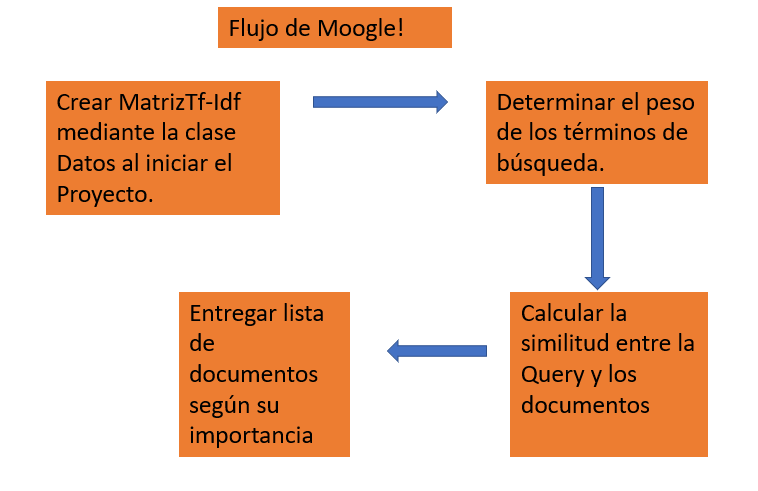
\includegraphics[width=12cm]{flujoM.png}
    \caption{Flujo del proyecto}
\end{figure}

\section{Conclusiones}
\begin{itemize}
    \item Éxito en la implementación del proyecto.
    \item Cumplimiento de los objetivos establecidos.
    \item Aprendizaje de nuevas herramientas y conceptos.
    \item Oportunidades de mejoras y trabajo futuro.
\end{itemize}

\end{document}